\graphicspath{{chapters/03/images/}}
\chapter{Implementation of the Stochastic Simulation Algorithms}

\section{Introduction}

  \subsection{Non-deterministic vs stochastic}
  Working under the assumption of using the same model and parameters:

  \begin{multicols}{2}
    \begin{itemize}
      \item A deterministic system does not show randomness and the same result is always obtained.
      \item A non-deterministic system shows some degree of uncertainty: different runs have different results.
    \end{itemize}
  \end{multicols}

    \subsubsection{Exact stochastic simulation}
    In an exact stochastic simulation, if some hypotheses are satisfied the system will behave like the biological one.
    Although the probability function could be computed, this does not make the method deterministic: uncertainty is intrinsic in the model.
    Theoretically there is no insight on the execution of the reactions in a stochastic setting, but a high level of accuracy can be reached thanks to the probability function.

  \subsection{Advantages of a non-deterministic approach}
  The reasoning behind the employment of a non-deterministic approach lies in the fact that to model a biological system there is a need to compromise between time and complexity.
  In non-deterministic polynomial time algorithms don't have an efficient solution, but it seems possible to find it.
  A non-deterministic setting allows us to understand whether an algorithm can be solved in polynomial time by step-wise guessing.

  \subsection{Categories of the exact simulation algorithms}
  A summary of the main exact stochastic simulation algorithms is reported in figure \ref{fig:tree}.

  \begin{figure}[H]
    \centering
    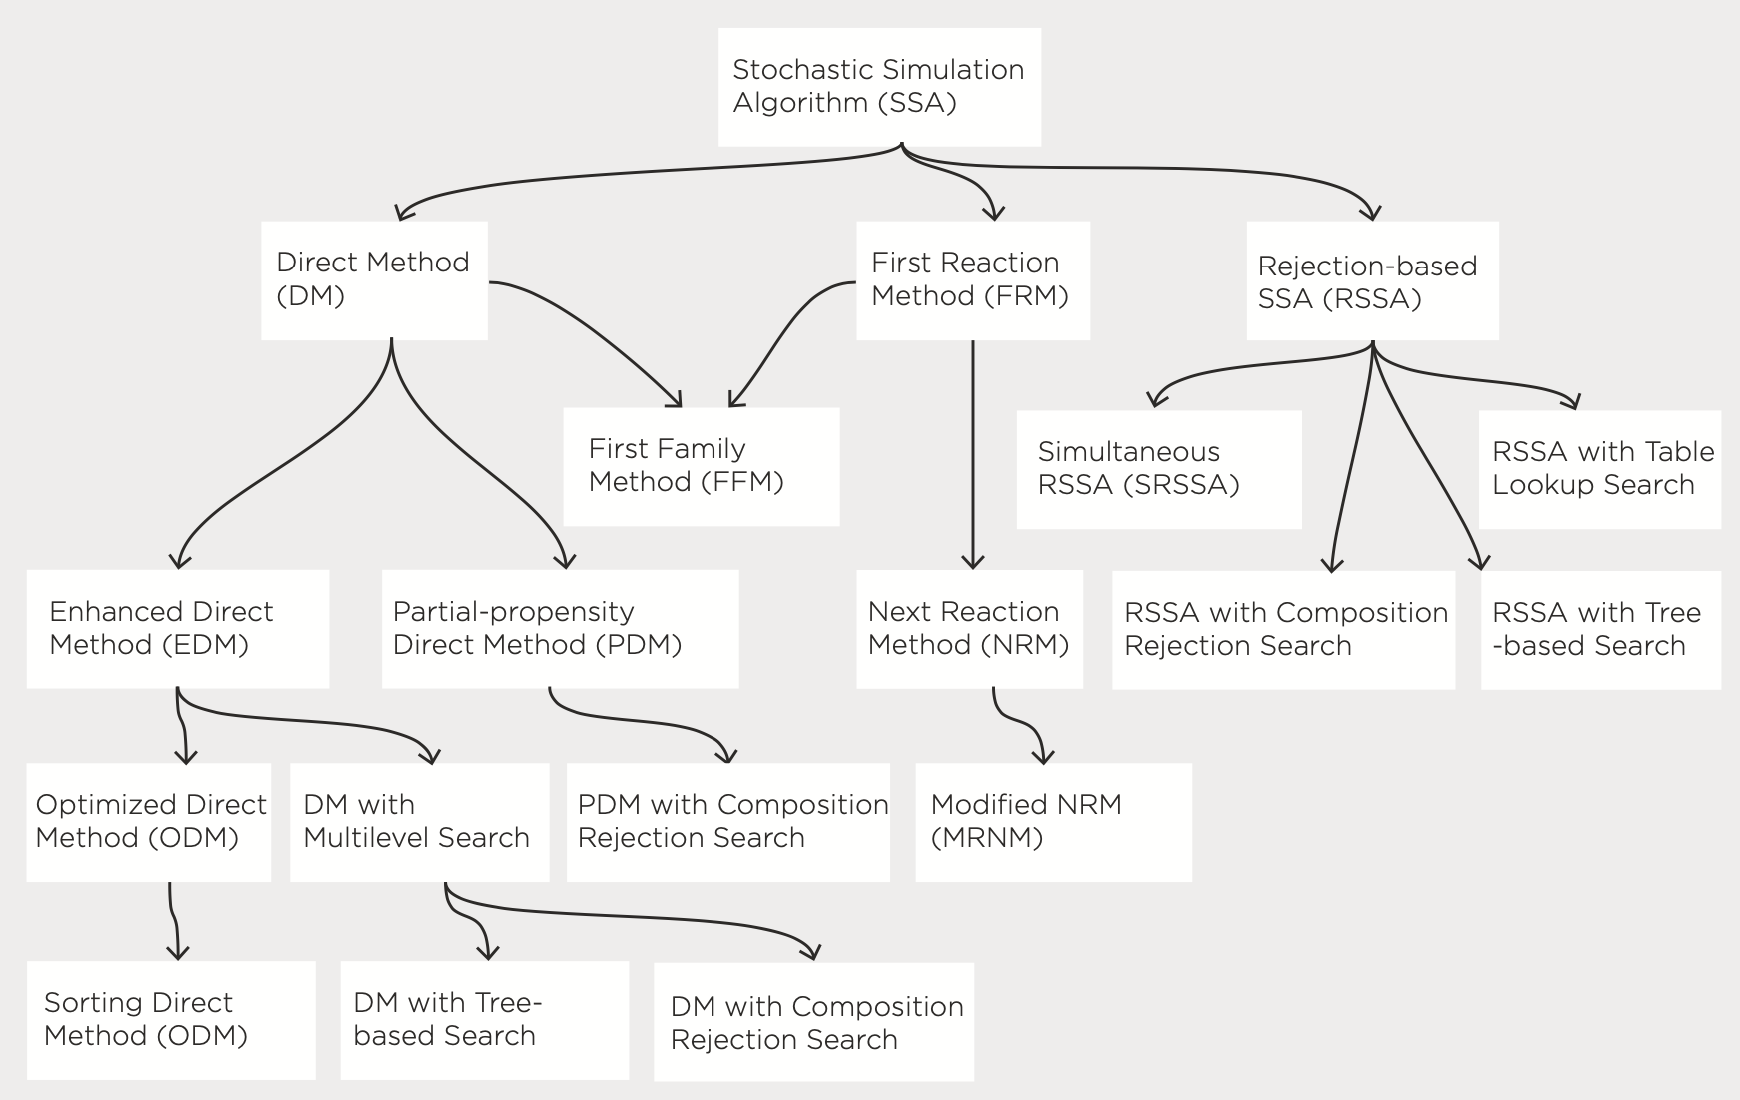
\includegraphics[width=\textwidth]{tree_methods.png}
    \caption{Fig 3.1 Marchetti's book}
    \label{fig:tree}
  \end{figure}

\section{Direct method}
Gillespie's direct method defines a couple of formulae able to understand how the system will execute in terms of time $\tau$ and reactions $\mu$.
Since each time step is infinitesimal each reaction occurs and ends exactly at time $\tau$, hence there cannot be multiple reactions firing simultaneously.
Let $a_0$ be the sum of all propensities in the system, then the algorithm works as follow:

\begin{enumerate}
  \item Sample one random number from the distribution $a_0 = \sum_{j=1}^{M}{a_j}\rightarrow V_1=U(0,1)$.
  \item Scale it to the maximum $V_1 \cdot a_0 =U(0,a_0)$.
  \item See where this number will point over the different propensities ( Figure \ref{fig:boundaries}).

    \begin{figure}[H]
      \centering
      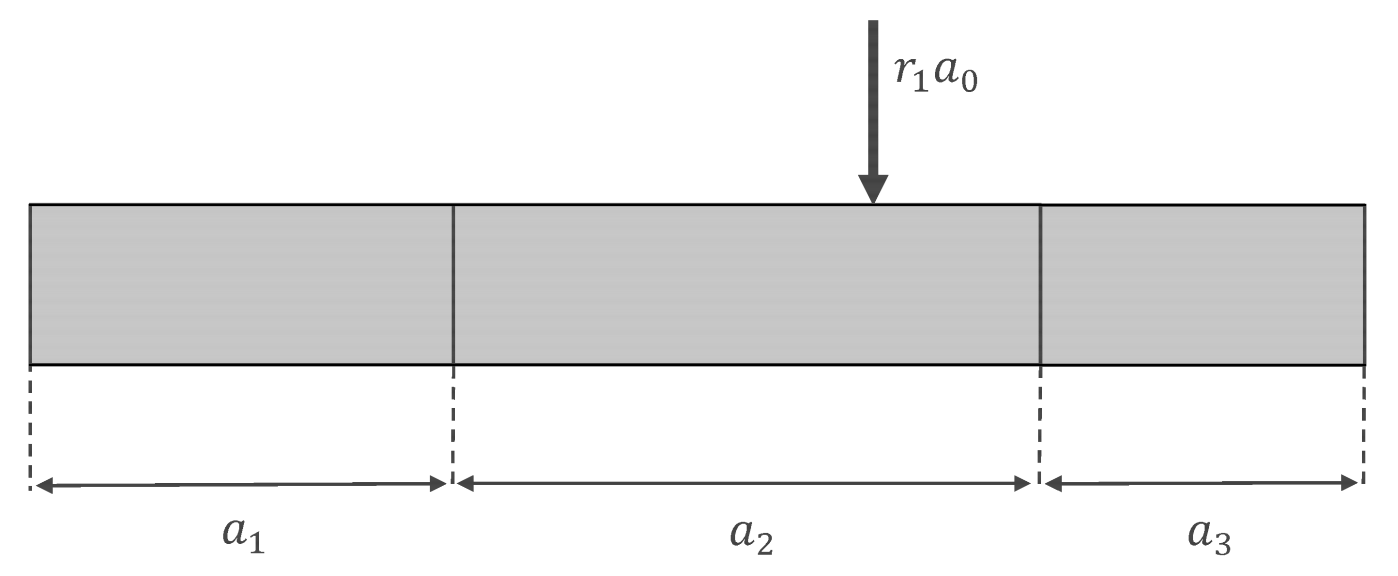
\includegraphics[width=\textwidth]{boundaries.png}
      \caption{Fig 3.2}
      \label{fig:boundaries}
    \end{figure}

  \item Generate another random number $V_2 =U(0,1)$ \item $\tau \sim Exp(a_0)$ \item $\tau = \frac{1}{a_0}ln(\frac{1}{V_2})$.
\end{enumerate}

  \subsection{Mathematical discussion}
  Gillespie's direct method is used to sample the pdf $p(\tau, \mu|\vec{x},t)$.
  The direct method partitions the joint probability density function into the product of two one-variable probability functions, one for $\tau$ and one for $\mu$ that can be sampled independently.
  The pdf can be factorized by the chain rule of probability as:

  $$p(\tau, \mu|\vec{x},t) = p_1(\tau|\vec{x},t)p_2(\mu|\vec{x},t)$$

  Where:

  \begin{multicols}{2}
    \begin{itemize}
      \item $p_1$ is the probability density function of the firing time $\tau$.
      \item $p_2$ is the probability density function of the reaction with index $\mu$ that fires at $t+\tau$.
    \end{itemize}
  \end{multicols}

  So that $p_1(\tau|\vec{x},t)d\tau$ is the probability that a reaction will fire in the next time interval $[t+\tau, t+\tau+d\tau[$.
  This marginal probability is obtained by summing the probability $p(\tau, \mu|\vec{x},t)d\tau$ over the domain of all possible values of reaction index $\mu$:

  $$p(\tau|\vec{x},t) = \sum\limits_{\mu=1}^Mp(\tau, \mu|\vec{x},t) = \sum\limits_{\mu=1}^Ma_\mu e^{a_0\tau} = a_0e^{-a_0\tau}$$

  Where $a_0$ is the total propensity.
  Plugging this and recalling the formula of the joint pdf:

  $$p_2(\mu|\tau,\vec{x},t) = \frac{p(\tau,\mu|\vec{x},t)}{p_1(\tau|\vec{x},t)} = \frac{a_\mu}{a_0}$$

  It can be seen how $p_2$ is independent of $\tau$, so it can be written as:

  $$p_2(\mu|\vec{x},t) = p_2(\mu|\tau,\vec{x},t) = \frac{a_\mu}{a_0}$$

  To verify that these two equation are part of the pdf:

  $$\int_0^{\infty}p_1(\tau|\vec{x},t)d\tau = \int_0^{\infty}a_0e^{-a_0\tau}d\tau = 1 \qquad\land\qquad \sum\limits_{\mu=1}^Mp_2(\mu|\vec{x},t) = \sum\limits_{\mu=1}^M\frac{a_\mu}{a_0} = 1$$

  The direct method uses $p_1(\tau|\vec{x},t)$ to sample the firing time $\tau$ and $p_2(\mu|\vec{x},t)$ to sample the reaction index $\mu$.
  Since the two pdfs are independent the firing time and the reaction index can be sampled independently, so that the order of sampling does not effect the exactness of the direct method.
  The generated firing time $\tau$ and the next reaction firing $R_\mu$ are ensured to have the pdf $p(\tau,\mu|\vec{x},t)$ specified by the stochastic simulation algorithm, so that the generated trajectories are exact.

    \subsubsection{Choice of the reaction}
    The selection of the next reaction index $\mu$ has probability $\frac{a_\mu}{a_0}$.
    Given $M$ discrete probabilities $\frac{a_j}{a_0}$ with $j = 1,\dots, M$, the choice of the next reaction index:

    \begin{align*}
      \mu &= \arg\min\limits_{\mu\in j=1,\dots,M}\sum\limits_{j=1}^M\frac{a_j}{a_0}\ge r_1 =\\
        &= \arg\min\limits_{\mu\in j=1,\dots,M}\sum\limits_{j=1}^Ma_j\ge r_1a_0
    \end{align*}

    Where $r_1$ is a uniformly distributed random number $norm(0,1)$.
    To select the next reaction firing $R_\mu$, the direct methods accumulates the sum $\sum\limits_{j=1}^\mu a_j$ until it finds the smallest index $\mu$ that satisfies that inequality.

    \subsubsection{Selection of the firing time}
    For the reaction of the firing time $\tau$, consider its pdf $p_1(\tau|\vec{x},t)$.
    It can be noted ho it is an exponential distribution with rate $a_0$.
    So the firing time can be generated as:

    $$\tau = \frac{1}{a_0}\ln\frac{1}{r_2}$$

    Where $r_2$ is a uniformly distributed random number $norm(0,1)$.

  \subsection{The algorithm}
  The independent sampling of the firing time and of the reaction index are the basis of each simulation step of the direct method, outlined in algorithm \ref{algo:dm}.

  \begin{algorithm}[H]
\DontPrintSemicolon
\SetKwComment{comment}{$\%$}{}
\SetKw{Int}{int}
\SetKw{To}{to}
\SetKw{Return}{return}
\SetKw{Not}{not}
\SetKw{Input}{Input}
\SetKw{Output}{Output}
\SetKwData{Item}{item}
\SetKwFunction{Min}{min}
\SetKwFunction{TitleFunction}{Direct Method (DM)}

\caption{\protect\TitleFunction{}}
\label{algo:dm}

\Input: a biochemical reaction network of $M$ reactions in which each reaction $R_j$, $j=1, \dots, M$ is accompanied with the state change vector $\vec{v}_j$ and the propensity $a_j$, the initial state $\vec{x}_0$ at time $0$ and the simulation ending time $T_{\max}$\;

\Output: a trajectory of the biochemical reaction network, which is a collection of states $X(t)$ for time $0\le t\le T_{\max}$\;

$t = 0$\;
$\vec{X} = \vec{x}_0$\;

\While{$t<T_{\max}$}{
	$a_0 = 0$\;
	\ForEach{$R_j$}{
		compute $a_j$\;
		$a_0 = a_0+a_j$\;
	}
	generate two random numbers $r_1,r_2\sim norm(0,1)$\;
	select $R_\mu$ with the smallest index $\mu$ such that $\sum\limits_{j=1}^\mu a_j\ge r_1a_0$\;
	$\tau = \frac{1}{a_0}\ln\frac{1}{r_2}$\;
	$\vec{X} = \vec{X}+\vec{v}_\mu$\;
	$t=t+\tau$\;
}

\end{algorithm}


  Lines $10$-$12$ implement the sampling of the joint reaction probability density function of the next reaction firing and its firign time.
  The simulation needs two random number, the first is used to select the next reaction firing with probability $\frac{a_\mu}{a_0}$, while the second for the firing tiem.
  The state is then advanced to the new one and the time is moved to $t+\tau$.

    \subsubsection{Time complexity}
    The computational cost for the generation of random numbers, the firing time and the update of simulation time are constant.
    Moreover the update of the state can be considered constant as only a few species are involved in a reaction.
    Because of this the computational cost of the algorithm arises due to:

    \begin{multicols}{2}
      \begin{itemize}
        \item The computation of reaction propensities due to state changes at lines $7$-$9$.
        \item The selection of the next reaction firing at line $11$.
      \end{itemize}
    \end{multicols}

    The direct method computes $M$ reaction propensities for each simulation step, so the time complexity for this step is of $O(M)$.
    The search for the next reaction in the worst case requires to sum up all the $M$ reaction propensities, making the cost for searching the next reaction firing $O(M)$.
    Summing up the time complexity for each simulation step of the direct method is $O(M)$.

  \subsection{Enhanced direct method}
  The enhanced direct method EDM reduces the number of propensity computation for each simulation iteration, recomputing only the propensity of reactions that change.
  The detection of changes in the reaction propensity is based on the fact that the propensity of a reaction changes only when the population of the reactants involved in the reaction changes only then the population of the reactants involved are changed by the reaction firing.
  Only the propensity of reaction that have reactant population changed are recomputed.
  This is decided by analysing the dependency relationship between reactions.

    \subsubsection{Reaction dependency graph}
    A reaction $R_j$ is dependent on a reaction $R_\mu$ if its propensity $a_j$ is changed when $R_\mu$ fires.
    This relationship is collected and presented in a reaction dependency graph.

      \paragraph{Some definitions}

        \subparagraph{Reactants and products set}
        For each reaction $R_j$, with $j = 1,\dots M$, define:

        $$Reactants(R_j) = \{S_i|S_i\text{ is a reactant of }R_j\}\qquad\land\qquad Products(R_j) = \{S_i|S_i\text{ is a product of }R_j\}$$

        \subparagraph{Affects set}
        The set of species involved in the computation of the propensity $a_j$ of a reaction $R_j$ is:

        $$Affects(R_j) = \{S_i|a_j\text{ changes if population of }S_i\text{ changes}\}$$

        \subparagraph{Mass action kinetics}
        For mass action kinetics, because the mass action propensity $a_j$ of reaction $R_j$ is proportional to its reactants:

        $$Affects(R_j) = Reactants(R_j)$$

        \subparagraph{AffectedBy set}
        The set of species whose population changes by firing reaction $R_j$ is:

        $$AffectedBy(R_j) = \{S_i|\text{Population of }S_i\text{ is changed if firing }R_j\}$$

        \subparagraph{Population of AffectedBy}
        For each reaction $R_j$ it is:

        $$AffectedBy(R_j)\subseteq Reactants(R_j)\cup Products(R_j)$$

        This is because $AffectedBy(R_j)$ includes species that are consumed and produced by reaction $R_j$ excluding any species whose population is conserved.

      \paragraph{Definition of the reaction dependency graph}
      Let $\mathcal{R}$ be the set of reactions in the biochemical reaction network.
      The reaction dependency graph $G(V, E)$ is a directed graph with the vertex set $V = \mathcal{R}$ and the edge set $E$ contains directed edges $e(R_j, R_k)$ from a reaction $R_j$ to another reaction $R_k$ if:

      $$AffectedBy(R_j)\cap Affects(R_k)\neq\emptyset$$

      All self-edges $e(R_j, R_j)$ belong to $E$.

      \paragraph{Dependent reactions}
      The set of reactions that are dependent on reaction $R_j$ by the reaction dependency graph $G$ is defined such that:

      $$Dependents(R_j) = \{R_k|\exists\text{ a directed edge }e(R_j,R_k)\in G\}$$

      The reaction dependency graph $G$ determines the reaction for which propensities must be recomputed after firing.
      The number of reaction in the $Dependents$ set is equal to the out-degree of the reaction in the dependency graph.

    \subsubsection{Algorithm}
    In the EDM algorithm the reaction dependency graph is the first thing built.
    This will be a static structure independent on the time evolution of the system and will be stored with a cost $O(M^2)$.
    The computation of propensity of all the reaction is performed only at the beginning of the simulation.
    For each iteration the selection is the same as in DM, then the new propensity for each reaction $R_j\in Dependents(R_\mu)$ is computed.
    The algorithm is presented in \ref{algo:edm}.

    \begin{algorithm}[H]
\DontPrintSemicolon
\SetKwComment{comment}{$\%$}{}
\SetKw{Int}{int}
\SetKw{To}{to}
\SetKw{Return}{return}
\SetKw{Not}{not}
\SetKw{Input}{Input}
\SetKw{Output}{Output}
\SetKwData{Item}{item}
\SetKwFunction{Min}{min}
\SetKwFunction{TitleFunction}{Enhanced Direct Method (EDM)}

\caption{\protect\TitleFunction{}}
\label{algo:edm}

\Input: a biochemical reaction network of $M$ reactions in which each reaction $R_j$, $j=1, \dots, M$ is accompanied with the state change vector $\vec{v}_j$ and the propensity $a_j$, the initial state $\vec{x}_0$ at time $0$ and the simulation ending time $T_{\max}$\;

\Output: a trajectory of the biochemical reaction network, which is a collection of states $X(t)$ for time $0\le t\le T_{\max}$\;

build the reaction dependency graph $G$\;
$t = 0$\;
$\vec{X} = \vec{x}_0$\;
\ForEach{$R_j$}{
	compute $a_j$\;
	$a_0 = a_0+a_j$\;
}
\While{$t<T_{\max}$}{
	generate two random numbers $r_1,r_2\sim norm(0,1)$\;
	select $R_\mu$ with the smallest index $\mu$ such that $\sum\limits_{j=1}^\mu a_j\ge r_1a_0$\;
	$\tau = \frac{1}{a_0}\ln\frac{1}{r_2}$\;
	$\vec{X} = \vec{X}+\vec{v}_\mu$\;
	$t=t+\tau$\;
	\ForEach{$R_j\in Dependents(R_\mu)$}{
		compute $a_j^{new}$\;
		$a_0 = a_0 + (a_j^{new}-a_j)$\;
		$a_j = a_j^{new}$\;
	}
}

\end{algorithm}


    In this way the propensity updates become local.
    Let $D$ be the average number of reactions depending in a reaction, the cost of the propensity update for a simulation loop becomes $O(D)$, considering that $D<M$, so the propensity update in EDM is more efficient than in DM.

  \subsection{Improvements for Direct Method}

    \subsubsection{Direct method with sorted reaction}
    The principle of the direct method with sorted reaction is to reduce the search depth of the direct method by re-indexing reactions, reducing the search depth of reactions that happens more frequently, improving simulation performance.

      \paragraph{Optimized direct method}
      The optimized direct method reduces the average search depth of the next reaction firing.
      This is done because in many biochemical networks, some reactions fire much more frequently tan others.

        \subparagraph{Average search depth}
        The average search depth $S_m$ is the average number of operation performed for the selection of the next reaction firing:

        $$S_M = \frac{\sum\limits_{j=1}^Mjn_j}{\sum\limits_{j=1}^Mn_j}$$

        Where:

        \begin{multicols}{2}
          \begin{itemize}
            \item $j$ is the search index of reaction $R_j$.
            \item $n_j$ is the number of times that $R_j$ fires during the simulation.
          \end{itemize}
        \end{multicols}

        These two values are not known so to order the reactions $\langle n_j\rangle$ the average estimation of $n_j$ is used to order reaction.
        This is computed by some short pre-simulation runs.

        \subparagraph{Algorithm}
        Optimized direct method is implemented as in algorithm \ref{algo:odm}.

        \begin{algorithm}[H]
\DontPrintSemicolon
\SetKwComment{comment}{$\%$}{}
\SetKw{Int}{int}
\SetKw{To}{to}
\SetKw{Return}{return}
\SetKw{Not}{not}
\SetKw{Input}{Input}
\SetKw{Output}{Output}
\SetKwData{Item}{item}
\SetKwFunction{Min}{min}
\SetKwFunction{TitleFunction}{Optimized Direct Method (ODM)}

\caption{\protect\TitleFunction{}}

\Input: a biochemical reaction network of $M$ reactions in which each reaction $R_j$, $j=1, \dots, M$ is accompanied with the state change vector $\vec{v}_j$ and the propensity $a_j$, the initial state $\vec{x}_0$ at time $0$ and the simulation ending time $T_{\max}$\;

\Output: a trajectory of the biochemical reaction network, which is a collection of states $X(t)$ for time $0\le t\le T_{\max}$\;

build the reaction dependency graph $G$\;
perform a few DM pre-simulation runs to estimate $\langle n_j\rangle$ of each reaction\;
order reaction indices such that $j<k$ if $\langle n_j\rangle>\langle n_k\rangle$\;
\ForEach{$R_j$}{
	compute $a_j$\;
	$a_0 = a_0+a_j$\;
}
$t = 0$\;
$\vec{X} = \vec{x}_0$\;
\While{$t<T_{\max}$}{
	generate two random numbers $r_1,r_2\sim norm(0,1)$\;
	select $R_\mu$ with the smallest index $\mu$ such that $\sum\limits_{j=1}^\mu a_j\ge r_1a_0$\;
	$\tau = \frac{1}{a_0}\ln\frac{1}{r_2}$\;
	$\vec{X} = \vec{X}+\vec{v}_\mu$\;
	$t=t+\tau$\;
	\ForEach{$R_j\in Dependents(R_\mu)$}{
		compute $a_j^{new}$\;
		$a_0 = a_0 + (a_j^{new}-a_j)$\;
		$a_j = a_j^{new}$\;
	}
}

\label{algo:odm}
\end{algorithm}


        \subparagraph{Discussion}
        In the case of a fixed number of bits the sum of the biggest propensities placed in the front of the search list may be not enough to account for the rest: the reactions with very small propensity will never fire.
        Moreover the pre-simulation introduces an additional computational burden to the simulation.
        Moreover ODM assumes that the reaction order determined by the pre-simulation runs will characterize the long-term reaction behaviour, which could not be true.

      \paragraph{Sorting direct method}
      The sorting direct method SDM is a variant of ODM that does not use pre-simulation runs by maintaining an approximately sorted order of reaction.
      The ordering is built dynamically during the simulation run: the index of a reaction whenever it is selected to fire is dynamically bubbled up one step ahead in the reaction list.
      The reactions that have just occurred are put towards the top of the search list.

        \subparagraph{Algorithm}
        The sorting direct method is implemented as in algorithm \ref{algo:sdm}.

        \begin{algorithm}[H]
\DontPrintSemicolon
\SetKwComment{comment}{$\%$}{}
\SetKw{Int}{int}
\SetKw{To}{to}
\SetKw{Return}{return}
\SetKw{Not}{not}
\SetKw{Input}{Input}
\SetKw{Output}{Output}
\SetKwData{Item}{item}
\SetKwFunction{Min}{min}
\SetKwFunction{TitleFunction}{Sorting Direct Method (SDM)}

\caption{\protect\TitleFunction{}}

\Input: a biochemical reaction network of $M$ reactions in which each reaction $R_j$, $j=1, \dots, M$ is accompanied with the state change vector $\vec{v}_j$ and the propensity $a_j$, the initial state $\vec{x}_0$ at time $0$ and the simulation ending time $T_{\max}$\;

\Output: a trajectory of the biochemical reaction network, which is a collection of states $X(t)$ for time $0\le t\le T_{\max}$\;

build the reaction dependency graph $G$\;
\ForEach{$R_j$}{
	compute $a_j$\;
	$a_0 = a_0+a_j$\;
}
$t = 0$\;
$\vec{X} = \vec{x}_0$\;
\While{$t<T_{\max}$}{
	generate two random numbers $r_1,r_2\sim norm(0,1)$\;
	select $R_\mu$ with the smallest index $\mu$ such that $\sum\limits_{j=1}^\mu a_j\ge r_1a_0$\;
	$\tau = \frac{1}{a_0}\ln\frac{1}{r_2}$\;
	$\vec{X} = \vec{X}+\vec{v}_\mu$\;
	$t=t+\tau$\;
	\ForEach{$R_j\in Dependents(R_\mu)$}{
		compute $a_j^{new}$\;
		$a_0 = a_0 + (a_j^{new}-a_j)$\;
		$a_j = a_j^{new}$\;
	}
	\If{$\mu > 1$}{
		Swap $R_\mu$ and $R_{\mu-1}$ in the reaction list\;
	}
}

\label{algo:sdm}
\end{algorithm}


        \subparagraph{Discussion}
        The swapping step adds overhead to each simulation step, but it is negligible.
        SDM is thus suited to deal with the simulation of networks where the propensities change sharply.

    \subsubsection{Direct method with Multi-level search}
    The mani bottleneck of DM is that the search for next reaction firing is slow in large reaction models.
    The multi-level search is an effort to reduce the time complexity of DM for large systems.
    The search problem is divided into smaller sub-problem partitioning the $M$ reactions into $L$ groups $G_1, \dots, G_L$.
    Each group $G_l$ contains $k_l$ reactions.
    Let $a^l$ be the sum of propensities of reactions in group $G_l$:

    $$a^l = \sum\limits_{R_j\in G_l}a_j$$

    It is obvious that:

    $$a_0 = \sum\limits_{l=1}^L a^l$$

    The selection of the next reaction firing is in two steps.
    First a group $G_\alpha$ is selected with probability $\frac{a^\alpha}{a_0}$.
    Then the next reaction firing $R_\mu$ is selected with probability $\frac{a_\mu}{a^\alpha}$ conditioning on the selected group $G_\alpha$.

      \paragraph{Exactness of the multi level search}
      The next reaction $R_\mu$ in the group $G_\alpha$ that is selected by the multi-level search has probability $\frac{a_\mu}{a_0}$.
      Let $\mathbb{P}\{R_\mu\}$ be the probability of selecting the reaction $R_\mu$.
      This can be expanded as:

      $$\mathbb{P}\{R_\mu\} = \mathbb{P}\{G_\alpha\}\mathbb{P}\{R_\mu|G_\alpha\} = \frac{a^\alpha}{a_0}\frac{a_\mu}{a^\alpha} = \frac{a_\mu}{a_0}$$

      \paragraph{Implementation}
      An implementation to select the group index and the reaction index requires two random numbers:

      $$\alpha = \arg\min\limits_{\alpha\in l = 1, \dots, L}\sum\limits_{l=1}^\alpha a^l\ge r_1a_0$$

      And:

      $$\mu = \arg\min\limits_{\mu\in k = 1, \dots, M}\sum\limits_{\substack{k=1\\G_\alpha = \{R_j, \dots, R_{j+k\alpha}\}}}^\mu a_k\ge r_2 a^\alpha$$

      The need  for $r_2$ can be avoided by recycling $r_1$:

      $$\frac{r_1 a_0 -\sum\limits_{l=1}^{\alpha-1}a^l}{a^\alpha}$$

      Is a uniformly distributed random number.
      SO $r_1$ is rescaled to select the next reaction firing in the group.

      \paragraph{Algorithm}
      The direct method with multi-level search is implemented as in algorithm \ref{algo:dm-multi-level}.

      \begin{algorithm}[H]
\DontPrintSemicolon
\SetKwComment{comment}{$\%$}{}
\SetKw{Int}{int}
\SetKw{To}{to}
\SetKw{Return}{return}
\SetKw{Not}{not}
\SetKw{Input}{Input}
\SetKw{Output}{Output}
\SetKwData{Item}{item}
\SetKwFunction{Min}{min}
\SetKwFunction{TitleFunction}{Direct method with multi level search}

\caption{\protect\TitleFunction{}}

\Input: a biochemical reaction network of $M$ reactions in which each reaction $R_j$, $j=1, \dots, M$ is accompanied with the state change vector $\vec{v}_j$ and the propensity $a_j$, the initial state $\vec{x}_0$ at time $0$ and the simulation ending time $T_{\max}$\;

\Output: a trajectory of the biochemical reaction network, which is a collection of states $X(t)$ for time $0\le t\le T_{\max}$\;

build the reaction dependency graph $G$\;
partition $M$ reactions into $L$ groups $\{G_1, \dots, G_L\}$\;

\ForEach{$G_l$}{
	$a^l = 0$\;
	\ForEach{$R_j\in G_l$}{
		compute $a_j$\;
		$a^l = a^l+a_j$\;
	}
	$a_0 = a_0+a^l$\;
}
$t = 0$\;
$\vec{X} = \vec{x}_0$\;
\While{$t<T_{\max}$}{
	generate two random numbers $r_1,r_2\sim norm(0,1)$\;
	select $G_\alpha$ with the smallest index $\alpha$ such that $\sum\limits_{l=1}^\alpha a^l\ge r_1a_0$\;
	$r_1 = \frac{r_1 a_0 -\sum\limits_{l=1}^{\alpha-1}a^l}{a^\alpha}$\;
	select $R_\mu$ with the smallest index $\mu$ such that $\sum\limits_{\substack{k=1\\G_\alpha=\{R_j, \dots, R_{j+n}\}}}^\mu a_k\ge r_1a^\alpha$\;
	$\tau = \frac{1}{a_0}\ln\frac{1}{r_2}$\;
	$\vec{X} = \vec{X}+\vec{v}_\mu$\;
	$t=t+\tau$\;
	\ForEach{$R_j\in Dependents(R_\mu)$}{
		compute $a_j^{new}$\;
		$a^l = a^l + (a_j^{new}-a_j)$\;
		$a_j = a_j^{new}$\;
	}
}

\label{algo:dm-multi-level}
\end{algorithm}


      \paragraph{Discussion}
      To analyse the time complexity of the multi-level search assume that $M$ reactions are partitioned into $L = \left[\frac{M}{k}\right]$ groups and each group contains $k_l=k$ reactions.
      The time complexity has two parts:

      \begin{multicols}{2}
        \begin{itemize}
          \item Searching for a group $O\left(\frac{M}{k}\right)$.
          \item Searching for a reaction within the group $O(k)$.
        \end{itemize}
      \end{multicols}

      The total time complexity is then

      $$O\left(\frac{M}{k}\right) + O(k) = O(\max\left\{\frac{M}{k}, k\right\})$$

      The total time is minimized by taking $k = c\sqrt{M}$, so that the minimal time complexity per reaction event is $O(\sqrt{M})$.
      The multi-level search can be further expanded partitioning the groups into sub-groups, introducing the multi-dimensional search method.

    \subsubsection{Direct method with tree-based search}
    The tree-based search refines the multi-level search.
    The finest partitioning of reaction is when the lowest level has at most two reaction creating a binary tree structure.
    Each node has two children or zero and the leaves hold reaction propensity, while internal node hold the sums of the values in their child nodes.
    The root of the tree holds $a_0$.

      \paragraph{Dimension of a complete tree}
      A complete binary tree with $M$ leaves has $2M-1$ nodes.
      Let $P$ be the number of internal nodes.
      In a complete tree each internal node has two children, hence the number of edges is $2P$.
      Also the edges are $M+P-1$, so $P = M-1$, so in conclusion the number of nodes is $P+M = 2M-1$.

      \paragraph{Implementation of the tree}
      The tree can be implemented by an array with $2M-1$ elements.
      The number of reaction $M$ has to be even, and if it is not a dummy node with propensity $0$ is added to the end of the array.
      Algorithm \ref{algo:build-tree} outlines how the tree is built: it happens recursively from the leaves to the root, observing that a node in $i$ will have children in position $2i$ and $2i+1$.

      \begin{algorithm}[H]
\DontPrintSemicolon
\SetKwComment{comment}{$\%$}{}
\SetKw{Int}{int}
\SetKw{To}{to}
\SetKw{Return}{return}
\SetKw{Not}{not}
\SetKw{Input}{Input}
\SetKw{Output}{Output}
\SetKwData{Item}{item}
\SetKwFunction{Min}{min}
\SetKwFunction{TitleFunction}{build\_tree}

\caption{\protect\TitleFunction{position}}
\label{algo:build-tree}

\Input: an array TREE with $2M-1$ elements where elements from $M$ to $2M-1$ are filled with $M$ reaction propensities and a starting position.\;

\Output: The complete binary tree represented by the array TREE.\;

\If{position $<M$}{
	\TitleFunction{$2\cdot$position}\;
	\TitleFunction{$2\cdot$position$+1$}\;
	$TREE[position] = TREE[2\cdot position] + TREE[2\cdot position +1]$\;
}


\end{algorithm}


      \paragraph{Tree-based search}
      The tree-based search for the next reaction firing $R_\mu$ given $s = ra_0$ starts by selecting the next branch of the tree by comparing the search value $s$ with the value stored in the left child of the current node.
      Then the search selects the left branch if the value is less than the one stored in the left child of the node, otherwise the search chooses the right branch.
      If the right branch is selected the search value is subtracted by the value stored in the current node.
      This proceeds recursively until it reaches a leaf and the reaction stored in that leaf is returned with the correct probability $\frac{a_\mu}{a_0}$.
      This procedure is outlined in \ref{algo:search-tree}.

      \begin{algorithm}[H]
\DontPrintSemicolon
\SetKwComment{comment}{$\%$}{}
\SetKw{Int}{int}
\SetKw{To}{to}
\SetKw{Return}{return}
\SetKw{Not}{not}
\SetKw{Input}{Input}
\SetKw{Output}{Output}
\SetKwData{Item}{item}
\SetKwFunction{Min}{min}
\SetKwFunction{TitleFunction}{search\_tree}

\caption{\protect\TitleFunction{position, s}}
\label{algo:search-tree}

\Input: A complete binary tree represented by the array TREE, and integer position and a search value $s$\;

\Output: The leaf of the complete binary tree which stores the next reaction firing.\;

\If{position $\ge$}{
	\Return position\;
}
\ElseIf{$TREE[2\cdot position]\ge s$}{
	\TitleFunction{$2\cdot position$, $s$}\;
}
\Else{
	$s = TREE[position] - s$\;
	\TitleFunction{$2\cdot position+1$, s}\;
}


\end{algorithm}


      \paragraph{Updating the tree}
      The system is updated after the selected reaction fires.
      The nodes of the tree will update their propensity value.
      For each reaction depending on the reaction firing according to the dependency graph $G$, its new propensity is computed and the difference is propagated for every of their paths.
      To optimize this implementation, reactions dependent on each other should be placed as close as possible on the tree.
      This procedure is outlined in algorithm \ref{algo:update-tree}.

      \begin{algorithm}[H]
\DontPrintSemicolon
\SetKwComment{comment}{$\%$}{}
\SetKw{Int}{int}
\SetKw{To}{to}
\SetKw{Return}{return}
\SetKw{Not}{not}
\SetKw{Input}{Input}
\SetKw{Output}{Output}
\SetKwData{Item}{item}
\SetKwFunction{Min}{min}
\SetKwFunction{TitleFunction}{update\_tree}

\caption{\protect\TitleFunction{position, c}}
\label{algo:update-tree}

\Input: A complete binary tree represented by the array TREE.\;

\Output: The complete binary tree updated by the reaction firing.\;

$TREE[position] = TREE[position] + C$\;
\If{position is not root}{
	\TitleFunction{$\left\lfloor\frac{i}{2}\right\rfloor$, $c$}\;
}

\end{algorithm}


      \paragraph{Algorithm}
      The whole procedure is implemented in the algorithm \ref{algo:dm-tree}.

      \begin{algorithm}[H]
\DontPrintSemicolon
\SetKwComment{comment}{$\%$}{}
\SetKw{Int}{int}
\SetKw{To}{to}
\SetKw{Return}{return}
\SetKw{Not}{not}
\SetKw{Input}{Input}
\SetKw{Output}{Output}
\SetKwData{Item}{item}
\SetKwFunction{Min}{min}
\SetKwFunction{TitleFunction}{Direct method with tree-based search}

\caption{\protect\TitleFunction{}}
\label{algo:dm-tree}

\Input: a biochemical reaction network of $M$ reactions in which each reaction $R_j$, $j=1, \dots, M$ is accompanied with the state change vector $\vec{v}_j$ and the propensity $a_j$, the initial state $\vec{x}_0$ at time $0$ and the simulation ending time $T_{\max}$\;

\Output: a trajectory of the biochemical reaction network, which is a collection of states $X(t)$ for time $0\le t\le T_{\max}$\;

build the reaction dependency graph $G$\;

$t = 0$\;
$\vec{X} = \vec{x}_0$\;

\ForEach{$R_l$}{
	compute $a_j$\;
}

build $TREE$ structure for $M$ reaction propensities with \ref{algo:build-tree}\;

\While{$t<T_{\max}$}{
	generate two random numbers $r_1,r_2\sim norm(0,1)$\;
	select next reaction firing $R_\mu$ by algorithm \ref{algo:search-tree} with $s= r_1a_0$\;
	$\tau = \frac{1}{a_0}\ln\frac{1}{r_2}$\;
	$\vec{X} = \vec{X}+\vec{v}_\mu$\;
	$t=t+\tau$\;
	\ForEach{$R_j\in Dependents(R_\mu)$}{
		compute $a_j^{new}$\;
		update the TREE by algoritm \ref{algo:update-tree} with $c = a_j^{new}-a_j$\;
		$a_j = a_j^{new}$\;
	}
}

\end{algorithm}


      \paragraph{Discussion}
      The search and updated are related to the height of the tree, logarithmic in the number of reactions.
      So the total computational cost for each reaction event is $O(\log(M))$.

      \paragraph{Tree with optimal height}
      The computational cost for selecting the next reaction firing in a complete tree is not the optimal average-case performance.
      Let $C$ be a tree structure.

        \subparagraph{Average number of comparison}
        The average number of comparison performed during the search in tree $C$ is:

        $$T_m(C) = \sum\limits_{j=1}^Mw_jD_j$$

        Where:

        \begin{multicols}{2}
          \begin{itemize}
            \item $M$ is the total number of reactions in the leaves.
            \item $D_j$ is the depth of leaf $R_j$.
            \item $w_j$ is a weight related to the probability that reaction $R_j$ is selected to fire.
          \end{itemize}
        \end{multicols}

        \subparagraph{Complete tree}
        When the tree $C$ is complete the depth $D_j$ is the same for all $j$.
        This leads to the fact that picking a fast reaction requires the same computational power of picking a slow one, leading to a non-optimal $T_M(C)$.

        \subparagraph{Huffman tree}
        The minimization of $T_M(C)$ leads to the construction of the Huffman tree.
        The leaves in this type of tree with large propensity values will be closer than the leaves with small values.
        This is built by merging trees in a forest, populated initially by trees with one node.
        At each step the two trees with roots $p$ and $q$ having the smallest weight $w_p$ and $w_q$ are merged creating the new root $pq$ with weight $w_{pq} = w_p+w_q$.
        The process stops when only one tree is found such that $D_{pq} +1 = D_q=D_q$, where $p, q, pq$ are the nodes involved in a merge such hat:

        \begin{align*}
          T_M(C) &= \sum\limits_{\substack{j=1\\j\neq p,q}}^Mw_jD_j +w_pD_q =\\
                 &= \left(\sum\limits_{\substack{j=1\\j\neq p,q}}^Mw_jD_j + w_{pq}D_{pq}\right) + w_{pq}=\\
                 &= T_{M-1}(C)+w_{pq}
        \end{align*}

        This derivation allows to determine that the Huffman tree gives the minimum value of $T_M(C)$.
        This is proven by induction on $M$.
        Consider the base case with $M=2$, this is easy to check.
        By the inductive hypothesis, the Huffman tree for $M-1$ gives the optimum value for $T_{M-1}(C)$.
        Suppose by contradiction that the Huffman tree for $M$ is not optimal, so there is some tree having the total number of comparison $T'_{M}(C)$ such that $T'_M(C)<T_M(C)$.
        Without loss of generality the smallest weights are placed at the lowest level.
        Let $p$ and $q$ be the nodes with the smallest weights and label their parent $pq$.
        Using the derivation this gives:

        $$T'_{M-1}(C) +w_{pq}< T_{M-1}(C)+w_{pq}$$

        Then $T_{M-1}'(C)< T_{M-1}(C)$, contradicting the inductive hypothesis.

        \subparagraph{Building the Huffman tree}
        To build a Huffman tree an array with size $2M-1$ is considered and each node has two children.
        However $M$ does not need to be even.
        The leaves are between $M$ and $2M-1$.
        Each element in the array points to its left and right child and an additional field parent points to the parent of the node.
        To extract the nodes with minimal weights a binary heap is used, such that each element is $(i,w_i)$, where $i$ is the index of a node in the tree and the weight $w_i$ is used as the key for ordering the heap.
        A heap is a tree-based data structure that satisfies the heap property: the key of a parent node is smaller than the key of its child nodes.
        The implementation for this procedure is presented in algorithm \ref{algo:huffman}

        \begin{algorithm}[H]
\DontPrintSemicolon
\SetKwComment{comment}{$\%$}{}
\SetKw{Int}{int}
\SetKw{To}{to}
\SetKw{Return}{return}
\SetKw{Not}{not}
\SetKw{Input}{Input}
\SetKw{Output}{Output}
\SetKwData{Item}{item}
\SetKwFunction{Min}{min}
\SetKwFunction{Insert}{insert}
\SetKwFunction{TitleFunction}{build\_huffman\_tree}

\caption{\protect\TitleFunction{position}}
\label{algo:huffman}

\Input: an array TREE with $2M-1$ elements where elements from $M$ to $2M-1$ are filled with $M$ reaction propensities\;

\Output: The Huffman tree represented by the array TREE.\;

build binary heap $H$ with elements $(M, w_1),\dots, (2M-1, w_M)$ ordered according to $W_j$\;
\For{$position = M-1$ \To $1$}{
	extract top element $(p, w_p)$ from $H$\;
	extract top element $(q, w_q)$ from $H$\;
	$TREE[position].VALUE = TREE[p].VALUE + TREE[q].VALUE$\;
	$TREE[position].LEFT = p$\;
	$TREE[position].RIGHT = q$\;
	\Insert{position, $w_p+w_q$} into $H$\;
	$TREE[p].PARENT = position$\;
	$TREE[q].PARENT = position$\;
}
\end{algorithm}


        The same binary search and propagation update are applied to search and update the propensities of the reactions.

        \subparagraph{Selecting the weight}
        The weight function $w_j$ can be the propensity function $a_j$ because it allows to reduce the time spent to find the next reaction, however reaction firing could make the tree no longer optimal, so it should be rebuilt.
        To balance the expensive operation of re-building with the non-optimal tree, the non-optimal tree is used for some number of steps.
        The choice for this step number only affect performance and not exactness.
        There are two approaches to do so:

        \begin{multicols}{2}
          \begin{itemize}
            \item Fixed time tree rebuilding.
            \item Adaptive time tre rebuilding.
          \end{itemize}
        \end{multicols}

        \subparagraph{Fixed time tree rebuilding}
        In fixed time tree rebuilding the tree structure is built every $k$ steps.
        To predict the changes in the reaction propensities during the $k$ steps the weights can be modified assigning a higher weight to those reaction that are more likely to change.\\

          \textbf{Conflicts and Favours set}
          For a reaction $R_j$ define:

          $$Conflicts(R_j) = \{R_k|(R_j\in Dependents(R_k))\land(Reactants(R_k)\cap Reactants(R_j)\neq\emptyset)\}$$

          $$Favors(R_j) = \{R_k|(R_j\in Dependents(R_k))\land (Products(R_k)\cap Reactants(R_j)\neq\emptyset)\}$$

          \textbf{Dependency graph}
          In terms of the dependency graph:

          $$|Conflicts(R_j)| + |Favours(R_j)| = in\ degree\ of\ R_j$$

          \textbf{Estimating changes of propensity}
          After a reaction firing, the probability that $R_j$ will increase or decrease is estimated as $\frac{|Conflicts(R_j)}{M}$ or $\frac{|Favours(R_j)}{M}$.
          For $k$ simulation steps, the estimated weight of reaction $R_j$ is:

          $$w_j(a_j, k) = a_j + \alpha_1 k\frac{|Favours(R_j)|}{M} + \alpha_2 k\frac{|Conflicts(R_j)|}{M}$$

          Where $\alpha_1$ and $\alpha_2$ are parameters denoting the amount of average change.

        \subparagraph{Adaptive time tree rebuilding}
        In adaptive time tree rebuilding the tree is rebuilt when a significant change has occurred.
        To detect the abrupt change in propensities a predefined value $\delta$, the acceptance threshold defines the largest change which does not require an immediate tree rebuilding.
        The difference in propensity after a reaction $R_j$ firing is $c_j = a_j^{new}-a_j$.
        If $c_j \ge \delta$ the Huffman tree should be rebuilt.
        To account for many small changes a cumulative sum of all the propensity changes $s_j$ since the last rebuilt is computes and compared against the acceptance threshold to decide whether to rebuild the tree.

    \subsubsection{Direct method with composition-rejection search}
    The composition-rejection CR search employs the partitioning of reaction into groups, but the selection of the next reaction is performed through an acceptance-rejection sampling.
    The reactions are partitioned into $L$ groups so that $R_j\in G_l$ if $a_j$ satisfies $2^{u_l-1}\le a_j\le 2^{u_l}$ in which $u_l$ is selected such that $u_l=\lceil \log_2(a_j)\rceil$.
    If $a_{\min}$ and $a_{\max}$, the global minimum and maximum propensities, are known, then $L = \left\lceil\log_2\left(\frac{a_{\max}}{a_{\min}}\right)\right\rceil$ for the whole simulation.
    These two bounds on $a$ can be estimated through physical reasoning.
    Where this is not possible $L$ must be increased during the simulation.

      \paragraph{Search for the next reaction}
      Let $a^l = \sum\limits_{R_j\in G_l}a_j$ be the sum of the propensity in group $G_l$.
      The total propensity $a_0$ can be computed as:

      $$a_0 = \sum\limits_{l=1}^La^l$$

      The search is composed of two steps.

        \subparagraph{First step}
        In the first step a group $G_\alpha$ is selected with probability $\frac{a^l}{a_0}$.
        This can be performed accumulating values $a^l$ until the smallest index $\alpha$ is found such that:

        $$\sum\limits_{l=1}^\alpha a^l\ge r_1a_0$$

        The tree-based search can be applied to select the group.

        \subparagraph{Second step}
        The second step is done through an acceptance-rejection sampling with the chosen envelope $2^{u_\alpha}$.
        A random and uniform reaction index $\mu\in G_\alpha$ is computed: $\mu = [r_2|G_\alpha|]$, where $|G_\alpha|$ is the size of $G_\alpha$ and $r_2$ is a random number.
        The selected reaction is tested to accept with probability $\frac{a_\mu}{2^{u_\alpha}}$: a random number $r_3$ is generated and compared against $\frac{a_\mu}{2^{u_\alpha}}$.
        $r_2$ can be recycled noting that $r_3 = r_2|G_\alpha|-\mu$ is uniformly distributed in $[0,1]$.
        If $\frac{a_\mu}{2^{u_\alpha}}\le r_3$ holds, $R_\mu$ is accepted to fire.
        Otherwise the reaction is rejected and a new random reaction index is generated and the check is performed again.
        This is repeated until there is an accepted $R_\mu$.
        The acceptance probability is bound to $\frac{1}{2}$: $\frac{a_\mu}{2^{u_\alpha}}\ge \frac{1}{2}$ by definition.

      \paragraph{Algorithm}
      An implementation of this method is found in algorithm \ref{algo:dm-cr}
      The rejection test is repeated on average two times: the acceptance rate is bounded by $\frac{1}{2}$.
      Moreover after a reaction firing the propensity must be updated and it could be that a new reaction falls outside of the current bound, so it must be moved to an appropriate group.

      \begin{algorithm}[H]
\DontPrintSemicolon
\SetKwComment{comment}{$\%$}{}
\SetKw{Int}{int}
\SetKw{To}{to}
\SetKw{Return}{return}
\SetKw{Not}{not}
\SetKw{Input}{Input}
\SetKw{Output}{Output}
\SetKwData{Item}{item}
\SetKwFunction{Min}{min}
\SetKwFunction{TitleFunction}{Direct Method with Composition-Rejection Search}

\caption{\protect\TitleFunction{}}
\label{algo:dm-cr}

\Input: a biochemical reaction network of $M$ reactions in which each reaction $R_j$, $j=1, \dots, M$ is accompanied with the state change vector $\vec{v}_j$ and the propensity $a_j$, the initial state $\vec{x}_0$ at time $0$ and the simulation ending time $T_{\max}$\;

\Output: a trajectory of the biochemical reaction network, which is a collection of states $X(t)$ for time $0\le t\le T_{\max}$\;

$t = 0$\;
$\vec{X} = \vec{x}_0$\;
build the dependency graph $G$\;
partition $M$ reactions into $L$ groups $\{G_1, \dots, G_L\}$ such that $R_j\in G_l$ if $2^{u_l-1}\le a_j\le 2^{u_l}$\;

$a_0 = 0$\;

\ForEach{$G_l$}{
	$a^l = 0$\;
	\ForEach{$R_j\in G_l$}{
		compute $a_j$\;
		$a^l = a^l + a_j$\;
	}
	$a_0 =a_0 + a^l$\;
}

\While{$t<T_{\max}$}{
	generate a random number $r_1\sim norm(0,1)$\;
	select $G_\alpha$ with the smalles group index $\alpha$ such that $\sum\limits_{l=1}^\alpha a^l\ge r_1a_0$\;

	\Repeat{$r_2\le \frac{a_\mu}{2^{u_\alpha}}$}{
		generate a random number $r_2\sim norm(0,1)$\;
		$\mu = [r_2|G_\alpha|]$\;
		$r_2 = r_2|G_\alpha|-\mu$\;
	}
	generate a random number $r_3\sim norm(0,1)$\;
	$\tau = \frac{1}{a_0}\ln\frac{1}{r_2}$\;
	$\vec{X} = \vec{X}+\vec{v}_\mu$\;
	$t=t+\tau$\;
	\ForEach{$R_j\in Dependents(R_\mu)$}{
		update $a_j$\;
		\If{$a_j\not\in[2^{u_l-1},2^{u_l}]$}{
			move $R_j$ from $G_l$ to an appropriate $G_m$\;
			updated $a^l$ and $a^m$\;
		}
		\Else{
			update $a^l$\;
		}
		update $a_0$\;
	}
}

\end{algorithm}


      \paragraph{Discussion}
      The selected base $2$ in the partition can be chosen arbitrarily, with the dimension of groups and the number of rejections increasing with the base.
      Moreover efficient data structures are needed to implement the movement of reactions between groups: this should support dynamic memory allocation operation.
      In addition a hash table should be used to support fast lookup of a reaction in a group.
      For adding a reaction to a group, the group size is increased and the reaction is added at the end of the group.
      When deleting a reaction, the reaction at the end of the group replaces it and the group size is decremented.
      After each of this two operations, the hash table is updated.

        \subparagraph{Computational cost}
        The computational cost is composed by the search for the group, proportional to the number of groups $O(L)$ and the costo for selecting the next reaction, which is constant.
        Because the average number of rejection tests is bound by $2$, the time is $O(L)$ and is independent of the number of reactions $M$.
        If $L\ll M$ and is bounded by a small constant the search for the next reaction firing is $O(1)$.

  \subsection{Partial-propensity direct method}
  The partial propensity direct method PDM requires that reactions must be elementary and their propensities follow the mass action kinetics.
  Mass action propensities are factorized and the partial propensities related to common reactants are grouped to facilitate the selection of the next reaction firing.
  Let $\pi_j^i$ the partial propensity of a reaction $R_j$ with respect to reactant $S_i$, this is defined as the propensity per molecule of reactant $S_i$.

    \subsubsection{Partial propensities of elementary reactions}

    \begin{itemize}
      \item Synthesis reaction ($\emptyset$ → products): propensity $ a_j =c_j $ and partial propensity $\pi_j^0 = c_j$.
      \item Unimolecular reaction ($ S_i$ → products): propensity $ a_j = c_jX_i $ and partial propensity $\pi_j^i=c_j$.
      \item Bimolecular reaction ($ S_i + S_k$ → products): propensity $ a_j = c_jX_iX_k $ and partial propensity $\pi_j^i = c_jX_k$ and $\pi_j^{(k)} = c_jX_i$.
      \item Dimerization reaction ($2S_i$ → products): propensity $ a_j = \frac{1}{2}c_jX_i(X_i -1) $ and partial propensity $\pi_j^i = \frac{1}{2}c_j(X_i-1)$.
    \end{itemize}

    \subsubsection{Storing the partial propensities}
    The partial propensities related to a species $S_i$ are grouped into  a group $\Pi_i$, such that the structure:

    $$\Pi = \{\Pi_i\}_{i=0}^N$$

    Stores all of them and is a matrix implemented as an array of arrays.
    It has $N+1$ rows in which the i-th row stores the partial propensities related to species $S_i$, while the 0-th row stores all the partial propensities for synthesis reactions.
    In the case of a bimolecular reaction one of the two partial propensities has to be dropped.

      \paragraph{Minimizing updates}
      To minimize updates the partial propensities are stored with respect to the reactant involved in a larger number of reaction: before building $\Pi$, the species are re-indexed such that for each pair of them $S_i$ and $S_k$, $i<k$ if the number of reactions involving $S_i$ is greater than $S_k$.
      Then PDM stores partial propensity of a bimolecular reaction with respect to the reactant with smaller index.

    \subsubsection{Group-sum array}
    The sum $\Lambda_i = \Sigma_j\Pi_{i,j}$ gives the sum of partial propensities of reactions $R_j$ sharing common reactant $S_i$.
    This is the group-sum array and is used to store the sum of partial propensities in group.
    $\Omega_i = X_i\Lambda_i$, where $X_i$ is the population of $S_i$ will be the sum of propensities of reaction having species $S_i$ as the common reactant.
    The array $\Omega = \{\Omega_i\}_{i=0}^N$ to store the sum of propensities of gropus.
    The total propensity is computed as:

    $$a_0 = \sum\limits_{i=0}^N\Omega_i$$

    \subsubsection{Reaction lookup}
    A reaction is identified by the group index $i$ and the element $j$ in a group $\Pi_i$.
    To facilitate the lookup of a reaction given the element $j$, a lookup table $\mathbf{L}$ is used to store the reaction indices of corresponding partial propensities in $\Pi$.
    It has the same structure as $\Pi$ ans is implemented as an array of arrays.
    The index of reaction with element index $j$ in group $i$ of $\Pi$ is identified as $\mathbf{L}_{ij}$, moreover three additional lookup table are used to facilitate the update of $\Pi$, $\Lambda$ and $\Omega$ after a reaction firing:

    \begin{multicols}{2}
      \begin{itemize}
        \item $\mathbf{U}^{(1)}$ is an array of $M$ arrays in which array $j$ contains the indices of species involved in $R_j$.
        \item $\mathbf{U}^{(2)}$ is an array of $M$ arrays in which the array $j$ contains the amount of change in population of the corresponding species in $\mathbf{U}^{(1)}$.
        \item $\mathbf{U}^{(3)}$ is an array of $N$ arrays in which array $k$ contains pairs of group indices and element indices of all entry in $\Pi$ that depend on species $k$.
          Each element in the row $k$ is a pair denoting the partial propensity $\Pi_{i,j}$ dependent in $X_k$.
      \end{itemize}
    \end{multicols}

    \subsubsection{Selecting the reaction firing}
    PDM selects $R_\mu$ in two steps.
    Let $r_1$ b a uniformly distributed random number in $norm(0,1)$.

      \paragraph{First step}
      Search for the group index $p$, with $0\le p\le N$:

      $$p = \arg\min\limits_{i\in p}\sum\limits_{i=0}^p\Omega_i\ge r_1a_0$$

      \paragraph{Second step}
      Search for an element index $q$, with $q\ge 1$ such that:

      $$q = \arg\min\limits_{i\in q}\left(X_p\sum\limits_{j=1}^q\Pi_{p,j}+\sum\limits_{i=0}^p\Omega_i-\Omega_p\right)\ge r_1a_0$$

      Or:
      $$q = \arg\min\limits_{i\in q}\Pi_{o,j}\ge \Psi$$

      Where:

      $$\Psi = \frac{r_1a_0-\sum\limits_{i=0}^p\Omega_i+\Omega_p}{X_p}$$

      Then $p$ and $q$ are used to retrieve the reaction firing index $\mu = \mathbf{L}_{p,q}$.


























\section{First Reaction Method (FRM)}
Instead of computing one $\tau$, compute a $\tau$ for each reaction (Figure \ref{fig:tau}).
Example: $\tau_1 = Exp(a_1)=1/a_1ln(1/V_1)$.
We are assuming that no other reactions are firing in the middle.
We can generate M random numbers and end up with M $\tau$.
Then we choose the reaction with minimum $\tau$, which will be the first selected one.
$\mu= R_{\mu}\text{ st }\tau_{\mu}= \min_{j}\tau_j$

 \begin{figure}
    \centering
    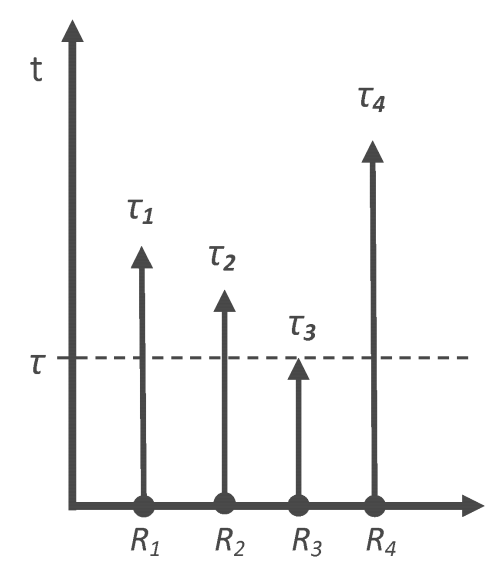
\includegraphics[width=0.3\textwidth]{R_tau.png}
    \caption{R Tau}
    \label{fig:tau}
  \end{figure}

\begin{itemize}
\item Pro: sometimes the search is quicker, simpler to parallelize.
\item Cons: we generate a lot of random numbers with respect to the direct method.
\end{itemize}

After the first step, we need to recompute. Even here, there is the possibility to improve the algorithm e.g.computation of the propensity.

\section{First Family Method}
Tries to combine the good features of the direct method with the first reaction method.
The idea is to reach an implementation which can be partially parallelizable: divide the reaction in ``families'' or groups.
The idea is to divide the reaction in n groups $r_1,…r_n$ and families e.g.~3 families.
We should associate a theoretical propensity to each group, i.e. the sum of the propensity in the family $a^1=\sum_{j\in f_1}a_j$.
$FRM= \tau_1= \frac{1}{e^1}ln(\frac{1}{r_1})$, we do not know which one of the reactions will be applied.
\\
\\
\noindent
In order to decide, we apply the direct reaction method formula for selecting the index.
Given that we are working with a subset, we will scale over the sum, the $a_0$ of the group.
It is true that we are generating random numbers, but over the number of the families → reduction.
This time we have n families + 1 random number to select the family.
Danger: if we have big disequilibrium in propensity, we might end up selecting always one of the families.
We can parallelize by linking families to CPU.
\\
\\
\noindent
Last time, we were introducing Next Reaction Method, which can be considered as an evolution, trying to apply the same reasoning as FRM in a more efficient way (by applying an efficient handling of random numbers).
If we are able to do so we will need to compute less random numbers.
DM → $2 \cdot n_{steps}$ FRM → $M \cdot n_{steps}$ FFM → $(n_{families}+ 1)n_{steps}$ NRM → $M+n_{steps}$.
If we take a look at the difference among methods, it is not very clear which is the winner - even though NRM seems to be one of the most optimized, it is usually the most efficient in requiring less random numbers.
Of course everything has a price, we need to add computations.
NRM is the most efficient in random number generation, while FRM is the one consuming the most.

\section{Next Reaction Method}
Why do we need to recompute time points? Two issues:

\begin{enumerate}
  \def\labelenumi{\arabic{enumi}.}
  \item multiple reactions can be executed at the same time → the reaction propensities might change \item we are computing $\tau$ over propensities, but the propensities were computed on initial reaction settings.
  E.g.$R_2:A \rightarrow B$, $R_1 : A \rightarrow B$ , the two reactions depend on each other.
\end{enumerate}

\noindent
$\tau$ is modelling the instant in which the reaction is assumed to fire, it is just an event.
We can subtract the time for passing to following reactions, but we must also update the propensity.
$a_1 \rightarrow a_1^{new}$, we have three possibilities:

\begin{enumerate}
  \def\labelenumi{\arabic{enumi}.}
  \item $a_1 = a_1^{new}$. $R_2$ is not affecting the propensity, i.e.~reactant is not modified by $R_2$, so $R_1$ remains unchanged.
  \item $a_2^{new}> a_1$. $R_2$ has been applied, something has changed and the firing prob of $R_1$ is increasing.
    Therefore, $\tau_1$ needs to be updated, we expect it to be smaller → rescaling through the ratio of the propensities e.g. ~$(\tau_1-\tau_2) \cdot \frac{a_1}{a_1^{new}}$ \item $a_1^{new}< a_2$ higher $\tau_1$
\end{enumerate}
\noindent
We should not think of another event, we are just updating the same event through the formula! The algorithm was developed in the 2000s, there are a lot of improvements related to technology advancements.
In addition to rescaling formula, there are other improvements to keep the complexity of the algorithm as low as possible:

\begin{itemize}
  \item we avoid generating too many random numbers
  \item reaction dependency graph (introduced for Direct Method): recompute the propensity of the reaction only if it is needed
  \item searching the reaction: minimum is linear over the number of reactions.
    \textbf{Binary heap}: decrease to logarithmic scale, select winner in constant time.
\end{itemize}
\noindent
Gibson 2000: original paper Thanh 2014: latest algorithm.

\section{RSSA}
The Rejection-based Simulation Algorithm seems to be an approximation, but everything is exact.
It tries to reduce computation complexity, but instead of limiting the amount of random numbers, it focuses on another bottleneck: the computation of the reaction propensity.
\\
\\
\noindent
The computational problem becomes more complex if we do not rely on mass action.
The RSSA Algorithm therefore tries to reduce the number of times in which we compute the reaction propensity.
We will need a placeholder and at the same time to keep the computation exact.
Instead of using the state of the system, we use a \textbf{\emph{fluctuation interval}}(a bound).
From the state of the system $X$ we generate a lower and upper bound; to do so, we just use a parameter providing a percentage, which is called $\delta$ ($0<\delta<1$).
Therefore, the bounds will be computed as:

\begin{itemize}
  \item lower $X = X - X \cdot \delta$ \item upper $X = X + X \cdot \delta$
\end{itemize}

\noindent
Given that the events of the reaction are modifying a few molecules per time, we can assume that for a certain amount of steps we will remain inside the same range of variability.
We are trying to obtain a propensity computed over bounds; by doing so, we can apply the same computation for a higher number of steps, as we only need to recompute the propensity outside of the fluctuation interval.
We can also compute the upper bound for the sum of the propensities $\bar{a}_0$.
$a_1$ will be in the middle, but we do not want to compute it.
It seems like working with these bounds does not lead to an exact simulation: we need to avoid as much as possible the exact computation of the propensities.
\\
\\
\noindent
Indeed, in the vast majority of cases we will have the possibility to choose the reaction without the real propensity.
We will perform some computations and, given the presence of bounds, we will do some mistakes; the algorithm will evaluate the results and eventually reject them (rejection-based algorithm).
For doing so, the algorithm generates the events with the upper bound of the propensity $\bar{a}_0$.
By using an upper bound $\tau$ will be lower, so we will generate more events with respect to the direct method.
We apply a sort of Gillespie, we replace the standard propensity with the upper bound and choose the reaction as in the direct method.
How can we understand whether an event is real or fake? In the case in which $\bar{a}_0 = a_0$ we are in the standard Gillespie.
We should apply a similar reasoning as NRM for scaling for checking the validity of candidate reactions.
\\
\\
\noindent
Let's imagine that we are selecting $R_2$: we should generate another random number, scale it over the bound and understand if we are in the exceeding (fake) or inside (real) area.

\begin{itemize}
  \item If the random number is lower than the lower bound, we can accept it without computing the real propensity.
  \item If the random number is between the bounds we require the exact propensity for discriminating:

  \begin{itemize}
    \item $\underline{a}_2 < u < a_2$ accept \item $a_2 < u < \bar{a}_2$ reject
  \end{itemize}

\end{itemize}

\noindent
The higher the fluctuation interval, the higher the uncertainty but lower the complexity → find the right compromise with some heuristics on $\delta$ value.
